%! TEX program = lualatex

% Gemini theme
% https://github.com/anishathalye/gemini

\documentclass[final]{beamer}

\pdfvariable inclusioncopyfonts=1

% ====================
% Packages
% ====================

\usepackage[T1]{fontenc}
\usepackage{lmodern}
\usepackage[scale=1.4]{beamerposter}

\setlength{\paperwidth}{48in}  
\setlength{\paperheight}{48in}    

\usetheme{gemini}
\usecolortheme{gemini}
\usepackage{graphicx}
\usepackage{booktabs}
\usepackage{tikz}
\usepackage{pgfplots}
\usepackage[export]{adjustbox}

\tolerance=1
\emergencystretch=\maxdimen
\hyphenpenalty=10000
\hbadness=10000

\usepackage[justification=justified]{caption}

% ====================
% Lengths
% ====================

% If you have N columns, choose \sepwidth and \colwidth such that
% (N+1)*\sepwidth + N*\colwidth = \paperwidth
\newlength{\sepwidth}
\newlength{\colwidth}
\setlength{\sepwidth}{0.025\paperwidth}
\setlength{\colwidth}{0.3\paperwidth}

\newcommand{\separatorcolumn}{\begin{column}{\sepwidth}\end{column}}

\makeatletter
\def\beamer@andinst{\quad}
\makeatother

 \addtobeamertemplate{block end}{}{\vspace*{-1.5cm}}

\newcommand{\eparzero}{\ensuremath{\mathring{E}(\text{PAR}, 0^+, t)}}
\newcommand{\micromol}{\textmu mol~m\textsuperscript{-2}~s\textsuperscript{-1}}
\newcommand{\kdparscalar}{\ensuremath{K_{\mathring{E}_d}}(\text{PAR})}
\newcommand{\eparscalar}{\ensuremath{\mathring{E}}(\text{PAR})}

\newcommand{\ppundericedevice}{\ensuremath{P_{\text{\scriptsize underice}}^{\text{\scriptsize device}}}}
\newcommand{\ppmixingdevice}{\ensuremath{P_{\text{\scriptsize mixing}}^{\text{\scriptsize device}}}}
\newcommand{\ppmixingsuit}{\ensuremath{P_{\text{\scriptsize mixing}}^{\text{\scriptsize SUIT}}}}
\newcommand{\ppundericedevicezt}{\ensuremath{P_{\text{\scriptsize underice}}^{\text{\scriptsize device}}(z,t)}}
\newcommand{\ppsuitunderice}{\ensuremath{P_{\text{\scriptsize underice}}^{\text{\scriptsize SUIT}}}}
\newcommand{\pprovunderice}{\ensuremath{P_{\text{\scriptsize underice}}^{\text{\scriptsize ROV}}}}
\newcommand{\ppopenwater}{\ensuremath{P_{\text{\scriptsize openwater}}}}
\newcommand{\ppmixing}{\ensuremath{P_{\text{\scriptsize mixing}}}}
\newcommand{\ppunderice}{\ensuremath{P_{\text{\scriptsize underice}}}}
\newcommand{\dailypp}{mgC~m\textsuperscript{-2}~d\textsuperscript{-1}}



% ====================
% Title
% ====================

\title{Sensitivity of phytoplankton primary production estimates to available irradiance under heterogeneous sea-ice conditions}

\author{P. Massicotte\inst{1,5}, I. Peeken\inst{2}, C. Katlein\inst{1,2}, H. Flores\inst{2}, Y. Huot\inst{3}, G. Castellani\inst{2}, S. Arndt\inst{2}, B. A. Lange\inst{2,4}, J.-É. Tremblay\inst{1,5} and M. Babin\inst{1,5}}


% \affiliation{1}{Takuvik Joint International Laboratory (UMI 3376) -- Université Laval (Canada) \& Centre National de la Recherche Scientifique (France)}
% \affiliation{2}{Alfred-Wegener-Institut Helmholtz-Zentrum für Polar- und Meeresforschung, Bremerhaven, Germany}
% \affiliation{3}{Université de Sherbrooke, Sherbrooke, Québec, Canada, J1K 2R1}
% \affiliation{4}{Fisheries and Oceans Canada, Freshwater Institute, Winnipeg, MB, Canada}
% \affiliation{5}{Québec-Océan et département de biologie, Université Laval, Québec, Canada, G1V 0A6}

\institute[shortinst]{\inst{1} Takuvik Joint International Laboratory, Université Laval \and \inst{2} Alfred-Wegener-Institut Helmholtz-Zentrum für Polar- und Meeresforschung \and \inst{3} Université de Sherbrooke \and \inst{4} Fisheries and Oceans Canada\and \inst{5} Québec-Océan et département de biologie, Université Laval}

% ====================
% Body
% ====================

\setbeamertemplate{bibliography entry article}{}

\begin{document}

\begin{frame}[t]
	\begin{columns}[t]
		\separatorcolumn

		\begin{column}{\colwidth}

			\begin{alertblock}{Take home messages}

				\begin{itemize}
					\justifying
					\setlength\itemsep{1em}
					\item Estimating primary production from photosynthetic parameters and transmittance measured at a single location does not provide a representative description of the spatial variability of the primary production occurring under a heterogeneous sea surface.
					\item Combining photosynthetic parameters measured in laboratory experiments with spatially representative transmittance values sampled with under-ice profiling platforms can significantly improve the accuracy of primary production estimates under heterogeneous sea surfaces.
					\item Spatially extensive in situ measurements must be combined with large-footprint sea-ice coverage sampling (e.g., remote sensing, aerial imagery) to accurately estimate primary production in ice-covered waters at larger scales.
				\end{itemize}
			\end{alertblock}


			\begin{block}{Problematics \& objectives}
				\begin{itemize}
					\justifying
					\setlength\itemsep{1em}
					\item During the last decades, the arctic icescape has been undergoing major changes, including a reduction of sea ice cover and thickness, and increased drift speed.
					\item Because of this surface heterogeneity, light transmittance can be highly variable in space, even over short distances.
					\item In such environments, phytoplankton is exposed to a highly variable light regime while drifting under a spatially heterogeneous. \textbf{Therefore, local irradiance measurements are not representative of the average irradiance experienced by phytoplankton over a large area.}
					\item \textit{Objective 1:} evaluate the potential of different underwater technologies to characterize the horizontal spatial variability of light transmittance at the ice-water interface (Figure 1).
					\item \textit{Objective 2:} use these transmittance data to assess the sensitivity of water-column primary production estimates to multi-scale under-ice light measurements.
				\end{itemize}

				\begin{figure}
					\centering
					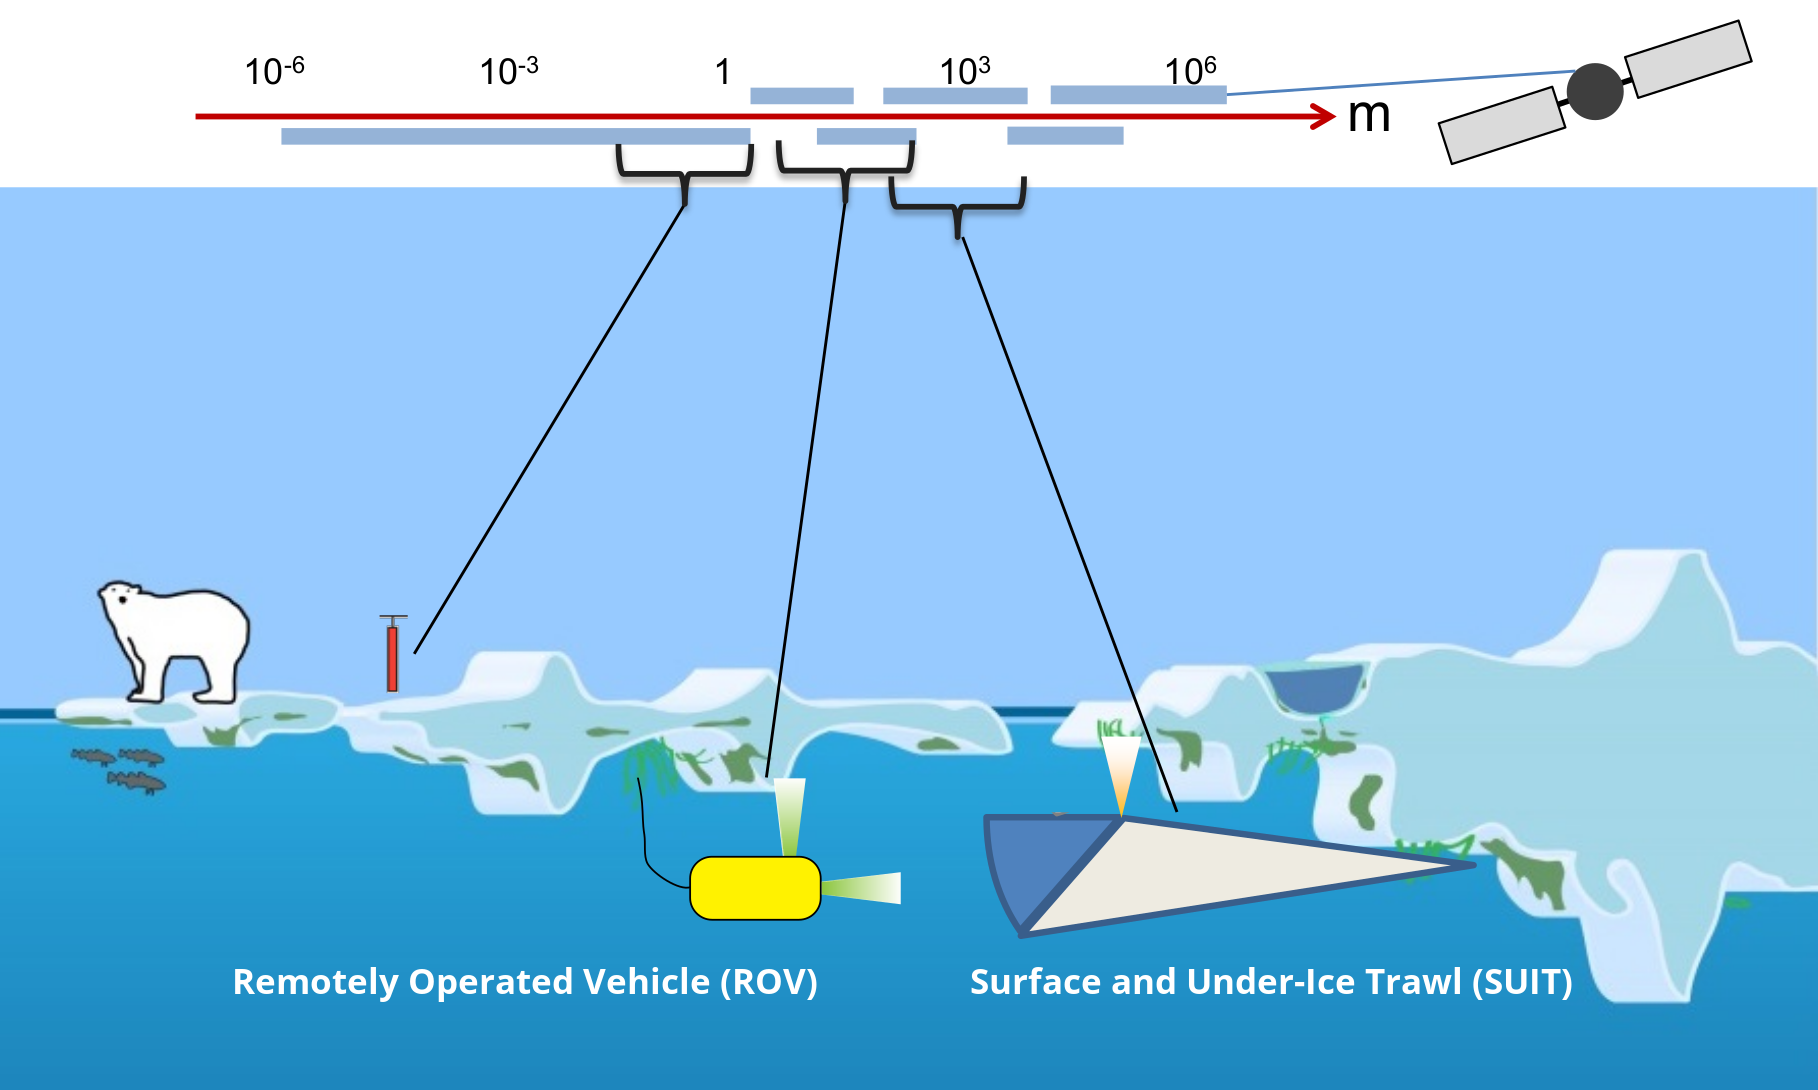
\includegraphics[scale = 0.75]{scales2.png}
					\caption{Schematic overview of spatial scales at which transmittance measurements were made by the ROV (hundreds of meters, deployed through a hole drilled through the ice) and the SUIT (thousands of meters, trawled behind an icebreaker).}
				\end{figure}

			\end{block}

			\vspace{3.5cm}
			\begin{minipage}[c]{0.175\textwidth}
				\includegraphics[scale = 0.5]{test3.eps}
			\end{minipage}
			\begin{minipage}[c]{0.75\textwidth}
				{\large \textbf{Download the poster by scanning the QR code!}}
			\end{minipage}

		\end{column}

		\separatorcolumn

		\begin{column}{\colwidth}

			\begin{block}{Key results}

				\textcolor{blue}{\large \textbf{ROV and SUIT transmittance measurements} (Figure 2)}

				\begin{itemize}
					\justifying
					\setlength\itemsep{1em}
					\item Transmittance values ranged between 0.001\% and 68\% for the ROV and between 0.002\% and 92\% for the SUIT.
					\item The transmittances measured by the SUIT were generally higher (mean = 35\%) by approximately one order magnitude than those measured with the ROV (mean = 2\%).
				\end{itemize}

				\begin{figure}
					\centering
					\includegraphics[scale = 2]{/media/work/projects/transsiz/graphs/fig3_poster.pdf}
					\caption{Density plots showing the distribution of transmittance values measured by the ROV and the SUIT devices. Dashed lines represent the 10\% transmittance threshold used to filter out SUIT transmittance used in the mixing models. Numbers on top of the gray boxes identify the stations. Top-left numbers in each facet show the number of observations.}
				\end{figure}

				\textcolor{blue}{\large \textbf{Estimated primary production} (Figure 3)}
				\begin{itemize}
					\justifying
					\setlength\itemsep{1em}
					\item Daily areal primary production derived from photosynthetic parameters and transmittance values ranged between 0.004 and 939 \dailypp{} for \ppunderice{} and between 0.004 and 731 \dailypp{} for \ppmixing{}.
					\item At stations 19 and 27, greater differences between \ppunderice{} and \ppmixing{} were observed in ROV-based estimates due to lower sea ice concentrations which allowed for a greater weight of \ppopenwater{} on the calculations.
				\end{itemize}

				\begin{figure}
					\centering
					\includegraphics[scale = 2]{/media/work/projects/transsiz/graphs/fig5_poster.pdf}
					\caption{Violin plots of primary production calculated from ROV and SUIT transmittance data. For SUIT data, mixing models were calculated using only transmittance~$\le$~10\% (see Figure 1) whereas the under-ice models were calculated using all transmittance data. Black dots inside the violin plots indicate the average primary production.}
				\end{figure}

			\end{block}

		\end{column}

		\separatorcolumn

		\begin{column}{\colwidth}

			\begin{block}{Key results (cont.)}

				\textcolor{blue}{\large \textbf{Error on primary production estimates} (Figure 4)}

				\begin{itemize}
					\justifying
					\setlength\itemsep{1em}
					\item The absolute relative errors ($\delta_P$) were distributed over a range covering four orders of magnitude, between 0.1\% and 1000\% which is corresponding to absolute primary production error varying between 0.0001 and 640 \dailypp{}.
					\item The lowest absolute errors (average $\approx$50\%) were associated with primary production estimates made using the mixing model approach (\ppmixing{}). Larger absolute errors were made with \ppunderice{} derived from only using ROV (mean = 88\%) and the SUIT (mean = 71\%) transmittances.
				\end{itemize}

				\begin{figure}
					\centering
					\includegraphics[scale = 2]{/media/work/projects/transsiz/graphs/fig6_poster.pdf}
					\caption{Distributions of the relative errors corresponding to the absolute deviation of each individual primary estimations from the average. The red lines and the numbers on the left indicate the mean errors.}
				\end{figure}

			\end{block}

			\begin{block}{\small Material \& methods}

				\footnotesize

				Process studies on biological productivity and ecosystem interactions were carried out north of Spitsbergen during the international Transitions in the Arctic Seasonal Sea Ice Zone (TRANSSIZ) expedition aboard the RV Polarstern (PS92, ARK-XXIX/1) between the 19th of May and the 26th June of 2015. In total, seven process studies (stations 19 27, 31, 39, 43, 46 and 47) were carried out where the ship was anchored to an ice floe, typically for 36 hours.

				\textcolor{blue}{\textbf{Light measurements \& estimating primary production}}

				\begin{itemize}
					\justifying
					\item Snow/sea-ice transmittance measurements were acquired at different spatial scales using a \textbf{Remotely Operated Vehicle, ROV} and a \textbf{Surface and Under-Ice Trawl, SUIT} (see Figure 1).
					\item Incident in-air downward photosynthetically active radiation, \eparzero{} (\micromol{}), was propagated into the water column using the downward diffuse attenuation coefficient of PAR calculated from the ROV.
					\item Primary production was then calculated using photosynthetic parameters derived from seawater samples incubated with 14\textsuperscript{C}-labelled sodium bicarbonate.
				\end{itemize}

				Two different approaches were used to calculate primary production from estimated photosynthetic parameters.

				\begin{itemize}
					\justifying
					\item \textit{Method 1: under-ice only primary production}: \eparscalar{} was propagated in the water column only under the ice using the transmittance values derived from either the ROV or the SUIT. Daily and depth-integrated primary production, \ppundericedevice{}, was calculated from transmittance measurements derived from both ROV and SUIT.
					\item \textit{Method 2: average production under ice and adjacent open waters} - The second approach consisted of using a mixing model, \ppmixingdevice{}, based on sea ice concentration (SIC) averaged over an area of $\approx$ 350 km\textsuperscript{2} derived from satellite imagery to upscale at a larger spatial scale the estimates of primary production derived from the ROV and the SUIT.
				\end{itemize}
			\end{block}

			\begin{block}{\small Acknowledgments}
				\footnotesize{We thank F. Bruyant, M. Beaulieu for carrying out the P vs. E curve measurements and providing us with the data. We thank Sascha Willmes for onboard processing of the ice and snow thickness data. We thank captain Thomas Wunderlich and the crew of icebreaker Polarstern for their support during the TRANSSIZ campaign (AWI\_PS92\_00). This study was conducted under the Helmholtz Association Research Programme Polar regions And Coasts in the changing Earth System II (PACES II), Topic 1, WP 4 and is part of the Helmholtz Association Young Investigators Groups Iceflux: Ice-ecosystem carbon flux in polar oceans (VH-NG-800). SUIT was developed by Wageningen Marine Research (WMR; formerly IMARES) with support from the Netherlands Ministry of EZ (project WOT-04-009-036) and the Netherlands Polar Program (project ALW 866.13.009). We thank Jan Andries van Franeker (WMR) for kindly providing the Surface and Under Ice Trawl (SUIT) and Michiel van Dorssen for technical support with work at sea. The project was conducted under the scientific coordination of the Canada Excellence Research Chair on Remote sensing of Canada's new Arctic frontier and the CNRS \& Université Laval Takuvik Joint International laboratory (UMI3376).}
			\end{block}
		\end{column}

		\separatorcolumn
	\end{columns}
\end{frame}

\end{document}
